\documentclass[12pt]{article}

\usepackage{amsmath,amsthm}
\usepackage{amsfonts}
\usepackage[psamsfonts]{amssymb}
\usepackage{palatino,euler}
\usepackage{graphicx}
\usepackage{hyperref}
\usepackage[french]{babel}
\usepackage{gensymb}
\usepackage{siunitx}

\begin{document}
\section{Impact de la profondeur}

En relation avec les travaux effectu\'es au Lac aux Castors, nous discuterons ici de l'effet de la
profondeur du plan d'eau sur les conditions de glace. En particulier, nous cherchons \`a savoir s'il est
possible que d'avoir creus\'e\cite{Lac} le lac \`a contribu\'e \`a la fermeture de la patinoire pour
assurer la s\'ecurit\'e du personnel et des citoyens.

\subsection{Hypoth\`eses}

Afin de d\'eterminer l'impact de la profondeur d'un plan sur la formation de la glace nous allons
encadrer la question des simplifications suivantes:

\begin{enumerate}
    \item Quoique la temp\'erature ext\'erieure va normalement varier suite \`a la contribution
        en chaleur du lac, nous allons consid\'erer que les variations locales vont se distribuer
        et traiter l'environnement ext\'erieur comme un puit de chaleur.
    \item Similairement pour l'apport du lac et de l'air \`a la temp\'erature du sol et allons
        donc traiter le sol comme une source de chaleur in\'epuisable;
    \item Nous n'allons \'evaluer que la perte d'\'energie du lac en terme de la conduction thermique
        et supposer que les contributions en radiation et \'evaporation\cite{Evap} des deux lacs est
        identique;
    \item Nous allons supposer la temp\'erature ext\'erieure constante. (Voir \ref{TempExt})
    \item Nous allons supposer la temp\'erature du sol constante et uniform\'ement distribu\'ee.
        (Voir \ref{Convec})
\end{enumerate}

Nous tenterons donc de d\'eterminer, pour un plan d'eau d'une surface de superficie fixe, de quelle fa\c
con une augmentation de la profondeur (et donc du volume d'eau) va prolonger la p\'eriode n\'ecessaire
pour refroidir le lac. On comparera donc deux corps d'eau id\'ealis\'es et d\'elimit\'es par la m\^eme
surface circulaire, l'un plus profond que l'autre.

\subsubsection{Temp\'erature ext\'erieure constante}\label{TempExt}

Pour obtenir une r\'eponse r\'ealiste nous aurions besoin d'une simulation ou d'une utilisation
judicieuse de probabilit\'es pour inclure une variation \`a la temp\'erature. En particulier, nous
savons que la chaleur transmise est proportionnelle \`a la diff\'erence de temp\'erature entre les
deux corps\cite{Fourier} et il serait pr\'eferable de ne pas n\'egliger cette composante.

Notre intuition nous dit qu'un lac dont le volume d'eau est sup\'erieur verra sa temp\'erature
varier plus lentement et que la diff\'erence de temp\'erature sera plus grande lorsque la
temp\'erature ext\'erieure est basse. Toutefois il est important d'appr\'ecier que si tel est le
cas, lorsque la temp\'erature ext\'erieure passe au dessus de celle de nos deux lacs, la situation
est renvers\'ee et le lac dont le volume est inf\'erieur verra sa temp\'erature remonter plus
rapidement aussi.

Nous jugeons donc qu'il est raisonnable de supposer la temp\'erature ext\'erieure constante. Les
composantes de gains et pertes en chaleur d\^ues \`a la variation de temp\'erature vont possiblement
s'annuler. Si ce n'est pas le cas et que le lac plus profond a une diff\'erence de temp\'erature
avec l'ext\'erieure plus grande on aura tout de m\^eme une r\'eponse positive \`a la question (que
le lac plus profond prends plus de temps \`a geler) en ayant possiblement sur\'estim\'e l'impact de
la profondeur.

\subsubsection{La convection thermique}\label{Convec}

Puisque nous \'evaluerons la diminution de la temp\'erature d'un lac par la chaleur fournie par le
plan d'eau \`a l'air environnant il s'ensuit que la temp\'erature chutera en surface. Comme nous le
verrons plus loin, la capacit\'e thermique\cite{CapTherm} massique du sol est inf\'erieure a celle
de l'eau, toutefois le volume de la terre est de loin sup\'erieur \`a celle d'un lac on pourra ainsi
supposer que la temp\'erature du sol va demeurer sup\'erieure \`a celle de l'eau par temps froid ce
qui justifie de traiter le sol comme une source de chaleur.

Nous allons par ailleurs supposer la temp\'erature du sol constante et uniform\'ement distribu\'ee.
Le sol \'etant un solide il n'est pas sujet \`a la convection tel l'eau du lac. Nous aurions
une meilleure approximation en consid\'erant le processus de diffusion qui, \`a un \'etat eventuel
stable, conduirait \`a une temp\'erature lin\'eairement distribu\'ee\cite{TempLinear}. Toutefois ces calculs seraient
compliqu\'es et nous pensons pouvoir d\'eduire, par le th\'eor\`eme de la moyenne\cite{AvgValue},
qu'il existe une temp\'erature constante pour laquelle la contribution en chaleur du sol sera la
m\^eme que pour une temp\'erature distribu\'ee de fa\c con plus r\'ealiste.

Une particularit\'e de l'eau est que la densit\'e de la phase solide est inf\'erieure \`a celle de
la phase liquide. De plus, la densit\'e de l'eau est maximale \`a
$\SI{3.98}{\celsius}$\cite{WaterDensity} ce qui introduit in\'evitablement un processus de
convection thermique\cite{ConvNat}. Aussi longtemps que la temp\'erature du lac est sup\'erieure \`a
$\SI{3.98}{\celsius}$ l'eau qui refroduit \`a la surface va sombrer et sera remplac\'ee par de l'eau
plus chaude provenant pr\`es de la terre l\`a o\`u la temp\'erature est plus \'elev\'ee.

\begin{figure}
    \centering
    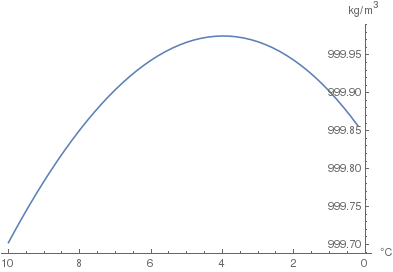
\includegraphics[scale=0.9]{WaterDensity.png}
    \caption{Densit\'e de l'eau}
\end{figure}

\clearpage
\begin{thebibliography}{Xyz}
    \bibitem{Lac}
        \href{https://www.ledevoir.com/politique/montreal/517828/patinoire-du-lac-aux-castors}
            {Montr\'eal abandonne la patinoire naturelle du lac aux Castors}
    \bibitem{Evap} \href{https://www.quora.com/How-does-evaporation-take-place-at-all-temperatures-whereas-boiling-takes-place-at-a-fixed-temperature-under-a-given-pressure}
        {How does evaporation take place at all temperatures}
    \bibitem{Fourier} \href{https://fr.wikipedia.org/wiki/Conduction_thermique#Loi_de_Fourier}
        {Loi de Fourier}
    \bibitem{CapTherm} \href{https://fr.wikipedia.org/wiki/Capacit%C3%A9_thermique_massique}
        {Capacit\'e thermique massique}
    \bibitem{TempLinear}
        \href{https://fr.wikipedia.org/wiki/Conduction_thermique#Surfaces_planes_en_série}
        {Conduction Thermique - Profil des temp\'eratures}
    \bibitem{AvgValue} \href{https://fr.wikipedia.org/wiki/Th%C3%A9or%C3%A8me_de_la_moyenne}
        {Th\'eor\`eme de la moyenne}
    \bibitem{WaterDensity} \href{http://www.open.edu/openlearn/science-maths-technology/the-oceans/content-section-3.2}
        {The density of fresh water and seawater}
    \bibitem{ConvNat} \href{https://fr.wikipedia.org/wiki/Convection_thermique#Convection_naturelle}
        {Convection naturelle}
    \bibitem{SpecHeat} \href{https://www.engineeringtoolbox.com/specific-heat-capacity-d_391.html}
        {Specific heat of common Substances}
\end{thebibliography}

\end{document}
